\section{Linux 平台下的基本命令}

作业中要求使用 Linux 平台进行操作，我使用一台阿里云 ECS 服务器完成实验。服务器配置为 2 核 2 GB，操作系统为 Ubuntu 24.04。本次实验通过 SSH 连接到服务器，并在真实 Linux 环境中完成命令演示。我使用 Termius 作为 SSH 客户端，便于在 Windows 电脑上远程连接服务器。

本节按照文件和目录、文件内容处理、系统信息、权限管理以及管道组合五类来整理命令。这样比单纯罗列命令更容易看出不同命令的使用场景，也能体现 Linux 命令之间可以组合使用的特点。

\begin{table}[H]
    \centering
    \caption{基础命令分类与实验目标}
    \small
    \begin{tabular}{p{0.20\textwidth} p{0.34\textwidth} p{0.30\textwidth}}
        \toprule
        命令类别 & 代表命令 & 实验目标 \\
        \midrule
        文件和目录 & \cmd{pwd}、\cmd{ls}、\cmd{mkdir}、\cmd{cp}、\cmd{mv}、\cmd{rm} & 熟悉路径、目录层次和文件生命周期操作 \\
        内容查看与处理 & \cmd{cat}、\cmd{head}、\cmd{tail}、\cmd{wc}、\cmd{sort}、\cmd{uniq}、\cmd{grep} & 学会从文本文件中查看、筛选、排序和统计内容 \\
        系统信息 & \cmd{uname}、\cmd{whoami}、\cmd{date}、\cmd{df}、\cmd{free}、\cmd{ps} & 观察当前 Linux 系统、资源和进程状态 \\
        权限管理 & \cmd{ls -l}、\cmd{chmod}、\cmd{stat} & 理解读、写、执行权限以及脚本可执行条件 \\
        管道组合 & \cmd{|}、\cmd{grep}、\cmd{sort}、\cmd{uniq}、\cmd{wc} & 把多个小工具组合成完整的数据处理流程 \\
        \bottomrule
    \end{tabular}
\end{table}

\subsection{文件和目录操作}

\begin{enumerate}
\item 查看当前所在目录：\cmd{pwd}
\item 查看当前目录下的文件：\cmd{ls}
\item 以详细形式查看文件：\cmd{ls -l}
\item 查看隐藏文件：\cmd{ls -a}

\begin{figure}[H]
    \centering
    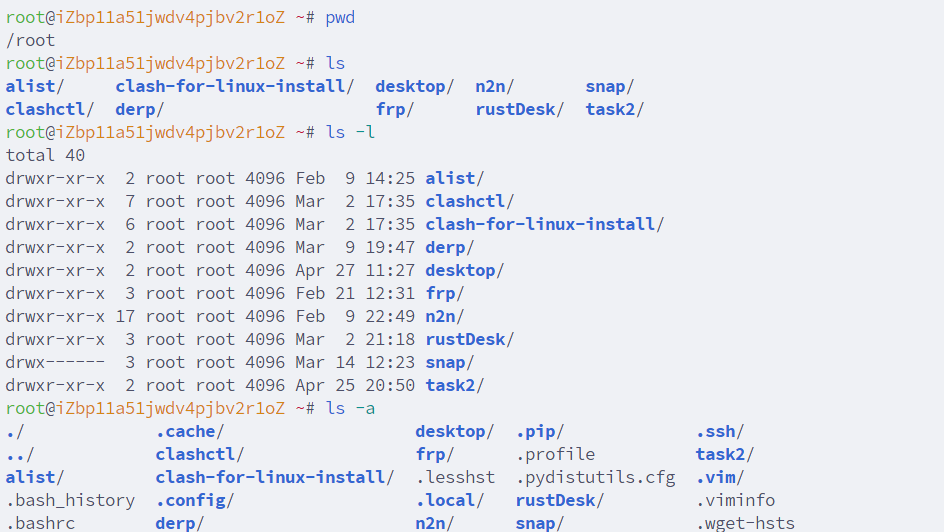
\includegraphics[width=0.8\textwidth]{pic/task1/image.png}
    \caption{命令1.1-1.4}
\end{figure}

\item 创建一个目录：\cmd{mkdir linux\_test}
\item 进入目录：\cmd{cd linux\_test}
\item 创建空文件：\cmd{touch file1.txt}
\item 向文件写入内容：\cmd{echo "hello linux" > file1.txt}
\item 查看文件内容：\cmd{cat file1.txt}
\item 复制文件：\cmd{cp file1.txt file2.txt}

\begin{figure}[H]
    \centering
    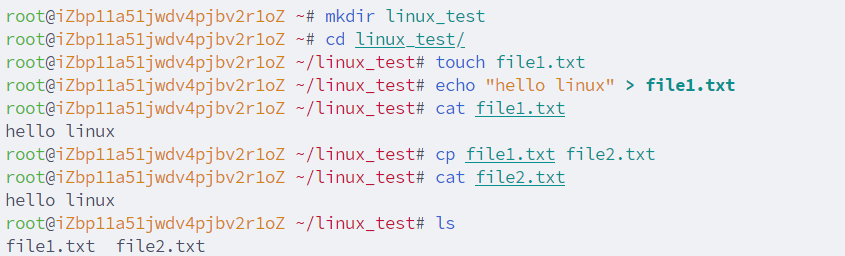
\includegraphics[width=0.8\textwidth]{pic/task1/image copy.png}
    \caption{命令1.5-1.10}
\end{figure}

\item 重命名文件：\cmd{mv file1.txt newfile.txt}
\item 删除文件：\cmd{rm newfile.txt}
\item 返回上一级目录：\cmd{cd ..}
\item 删除目录：\cmd{rm -r linux\_test}

\begin{figure}[H]
    \centering
    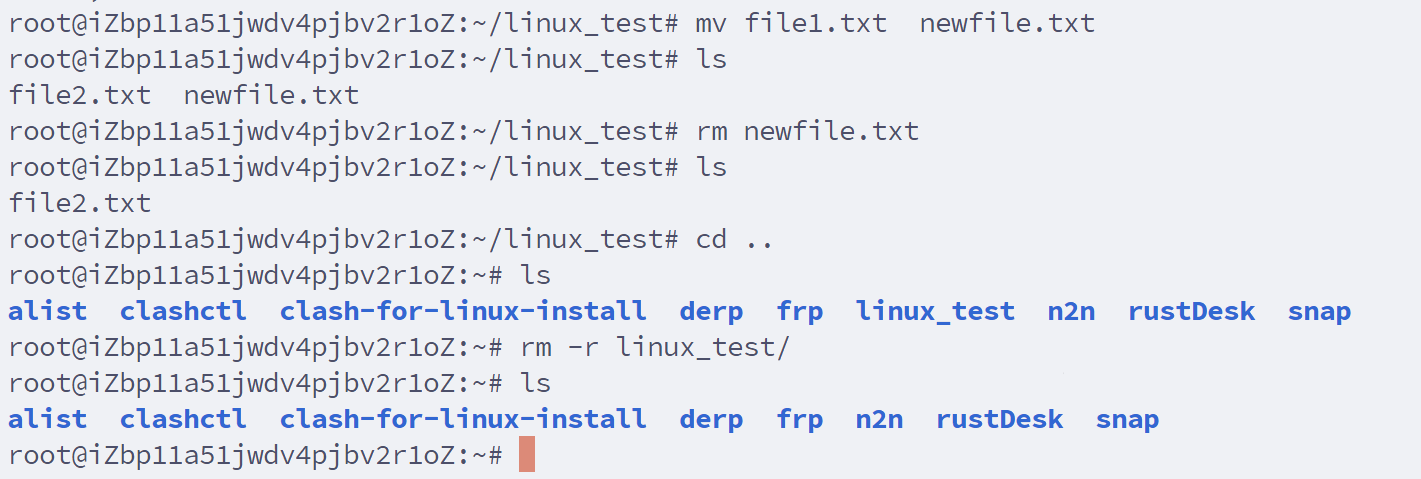
\includegraphics[width=0.8\textwidth]{pic/task1/image copy 2.png}
    \caption{命令1.11-1.14}
\end{figure}

\end{enumerate}

这一组命令展示了 Linux 中文件从创建、写入、复制、重命名到删除的完整过程。需要注意的是，\cmd{rm} 和 \cmd{rm -r} 都属于不可逆的删除操作，真实使用时应先通过 \cmd{pwd} 和 \cmd{ls} 确认当前目录和目标文件，避免在错误目录下删除内容。目录操作中，\cmd{cd ..} 表示返回父目录，\cmd{./} 表示当前目录，理解这些相对路径写法后，后续执行脚本和引用文件会更清晰。

\begin{table}[H]
    \centering
    \caption{文件目录命令使用要点}
    \small
    \begin{tabular}{p{0.18\textwidth} p{0.28\textwidth} p{0.36\textwidth}}
        \toprule
        命令 & 常用场景 & 注意点 \\
        \midrule
        \cmd{pwd} & 查看当前工作目录 & 执行删除、复制前先确认位置，避免误操作 \\
        \cmd{ls -la} & 同时查看详细信息和隐藏文件 & 以点号开头的文件默认不会被普通 \cmd{ls} 显示 \\
        \cmd{mkdir} & 创建项目目录或实验目录 & 如果父目录不存在，需要先创建父目录或使用合适路径 \\
        \cmd{cp} & 复制文件作为备份 & 复制目录时通常需要加 \cmd{-r} 参数 \\
        \cmd{mv} & 移动文件或重命名文件 & 同名目标可能被覆盖，执行前要确认目标路径 \\
        \cmd{rm -r} & 删除目录及其中内容 & 风险较高，实验中只对临时目录使用 \\
        \bottomrule
    \end{tabular}
\end{table}

\subsection{文件内容查看与处理命令}

我先使用如下命令创建测试目录和测试文件，然后再对文件内容处理命令进行演示。

\begin{minted}{bash}
mkdir linux_homework
cd linux_homework
echo -e "apple\nbanana\napple\norange\nbanana\nlinux\ncommand\npipe" > words.txt    
\end{minted}

\begin{enumerate}
\item 查看完整内容：\cmd{cat words.txt}

\begin{figure}[H]
    \centering
    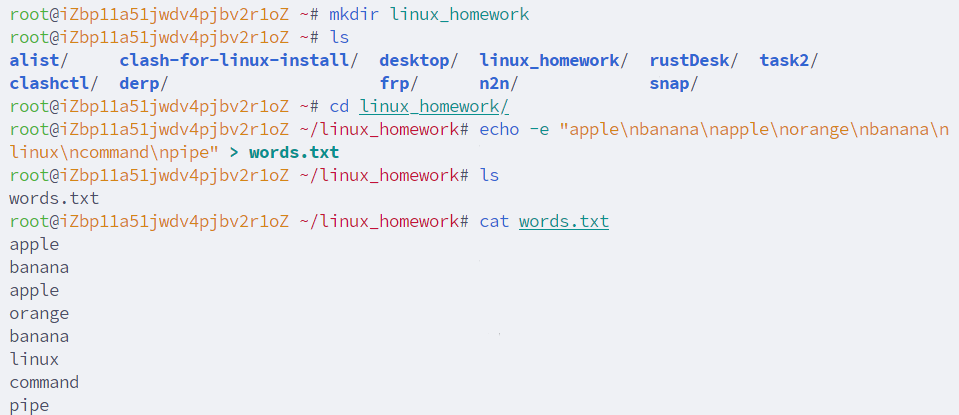
\includegraphics[width=0.8\textwidth]{pic/task1/image copy 3.png}
    \caption{命令2.1}
\end{figure}

\item 查看文件前3行：\cmd{head -n 3 words.txt}
\item 查看文件后3行：\cmd{tail -n 3 words.txt}
\item 统计文件行数、单词数、字符数：\cmd{wc words.txt}
\item 统计文件行数：\cmd{wc -l words.txt}
\begin{figure}[H]
    \centering
    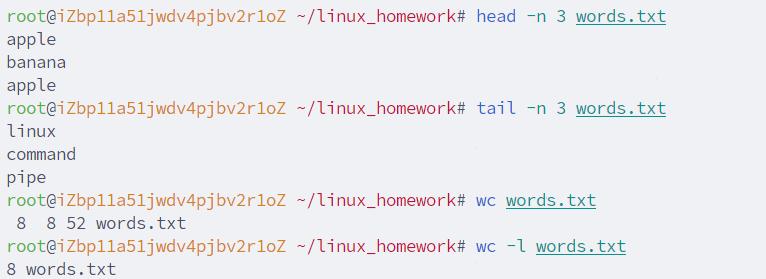
\includegraphics[width=0.8\textwidth]{pic/task1/image copy 4.png}
    \caption{命令2.2-2.5}
\end{figure}

\item 对文件内容排序：\cmd{sort words.txt}
\item 去除相邻重复行：\cmd{uniq words.txt}
\item 查找包含 apple 的行：\cmd{grep "apple" words.txt}
\item 查找包含 banana 的行，并显示行号：\cmd{grep -n "banana" words.txt}

\begin{figure}[H]
    \centering
    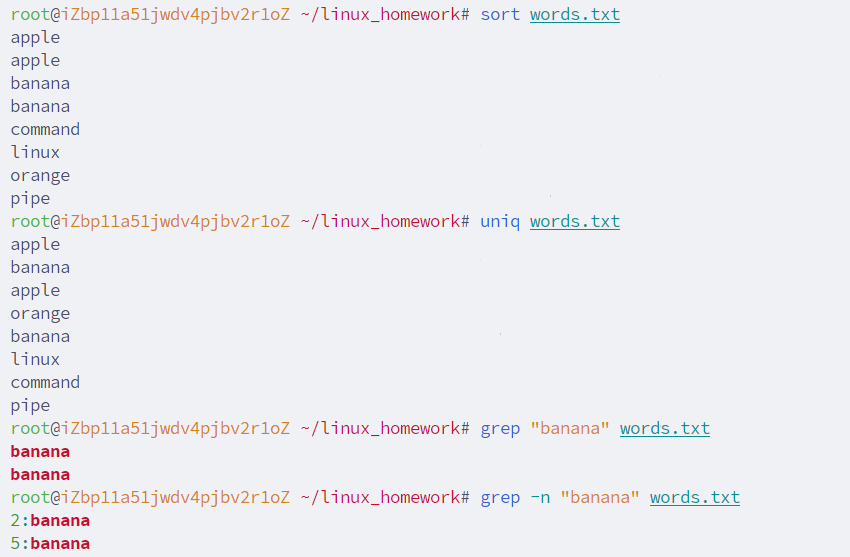
\includegraphics[width=0.8\textwidth]{pic/task1/image copy 5.png}
    \caption{命令2.6-2.9}
\end{figure}

\cmd{uniq} 只能去除相邻的重复行，如果重复内容之间隔着其他行，直接执行 \cmd{uniq words.txt} 并不能完成全局去重。因此在后面的管道命令中，我又使用 \cmd{sort words.txt | uniq}，先把相同内容排到相邻位置，再进行去重统计。

\end{enumerate}

文件内容处理命令体现了 Linux 把文本作为基础数据格式的特点。很多配置、日志、题库和脚本都可以被看作普通文本文件，因此掌握查看、筛选、统计和排序命令后，就可以在不打开图形化编辑器的情况下快速定位信息。例如查看日志时常用 \cmd{tail -n 50} 看末尾几十行，统计题库行数时可以使用 \cmd{wc -l}，从大量输出中查找关键词时可以使用 \cmd{grep}。

\begin{table}[H]
    \centering
    \caption{文本处理命令对比}
    \small
    \begin{tabular}{p{0.18\textwidth} p{0.30\textwidth} p{0.34\textwidth}}
        \toprule
        命令 & 适合解决的问题 & 本次实验中的体现 \\
        \midrule
        \cmd{cat} & 快速查看小文件完整内容 & 查看 \cmd{words.txt} 中的全部测试单词 \\
        \cmd{head} / \cmd{tail} & 只查看文件开头或结尾 & 验证文件前 3 行和后 3 行内容 \\
        \cmd{wc} & 统计行数、单词数和字符数 & 判断测试文件规模和行数 \\
        \cmd{sort} & 按字典序排列文本行 & 为去重和词频统计做准备 \\
        \cmd{uniq} & 合并相邻重复行 & 与 \cmd{sort} 配合完成全局去重 \\
        \cmd{grep} & 按关键词筛选文本行 & 查找包含指定单词的行，并显示行号 \\
        \bottomrule
    \end{tabular}
\end{table}

\subsection{系统信息查看命令}

\begin{enumerate}
\item 查看系统内核和系统信息：\cmd{uname -a}
\item 查看当前用户名：\cmd{whoami}
\item 查看当前日期时间：\cmd{date}
\item 显示日历：\cmd{cal}

\begin{figure}[H]
    \centering
    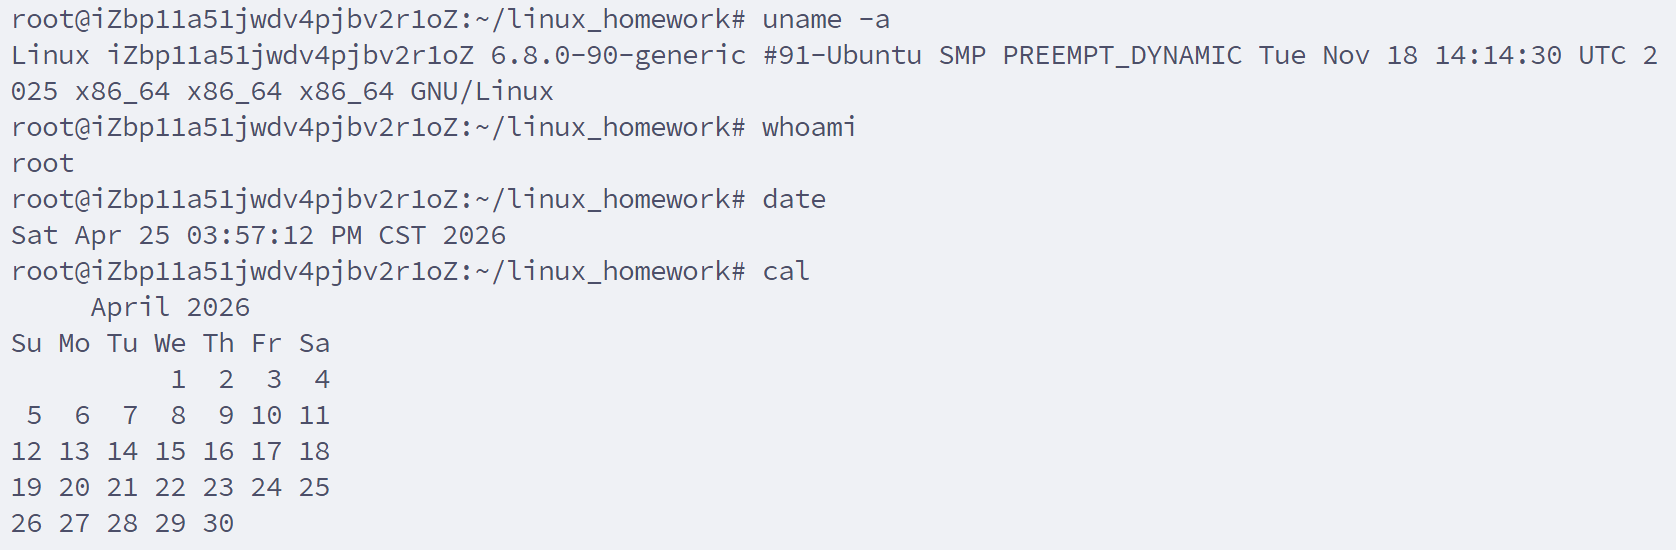
\includegraphics[width=0.8\textwidth]{pic/task1/image copy 6.png}
    \caption{命令3.1-3.4}
\end{figure}

如果系统默认没有安装 \cmd{cal} 命令，需要先安装 \cmd{ncal} 包。我使用 \cmd{sudo apt install ncal} 安装之后，就可以正常显示日历。

\item 查看磁盘空间：\cmd{df -h}
\item 查看内存使用情况：\cmd{free -h}

\begin{figure}[H]
    \centering
    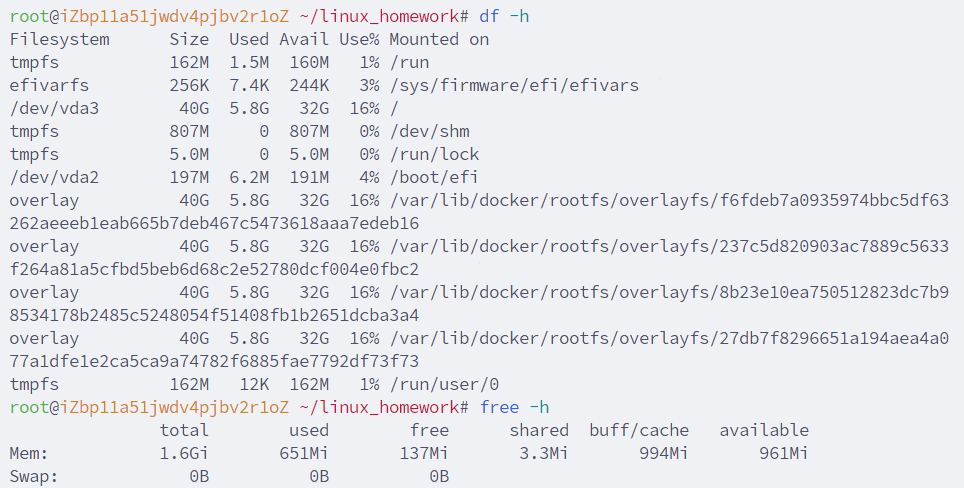
\includegraphics[width=0.8\textwidth]{pic/task1/image copy 7.png}
    \caption{命令3.5-3.6}
\end{figure}

\item 查看系统进程和资源占用：\cmd{top}

\begin{figure}[H]
    \centering
    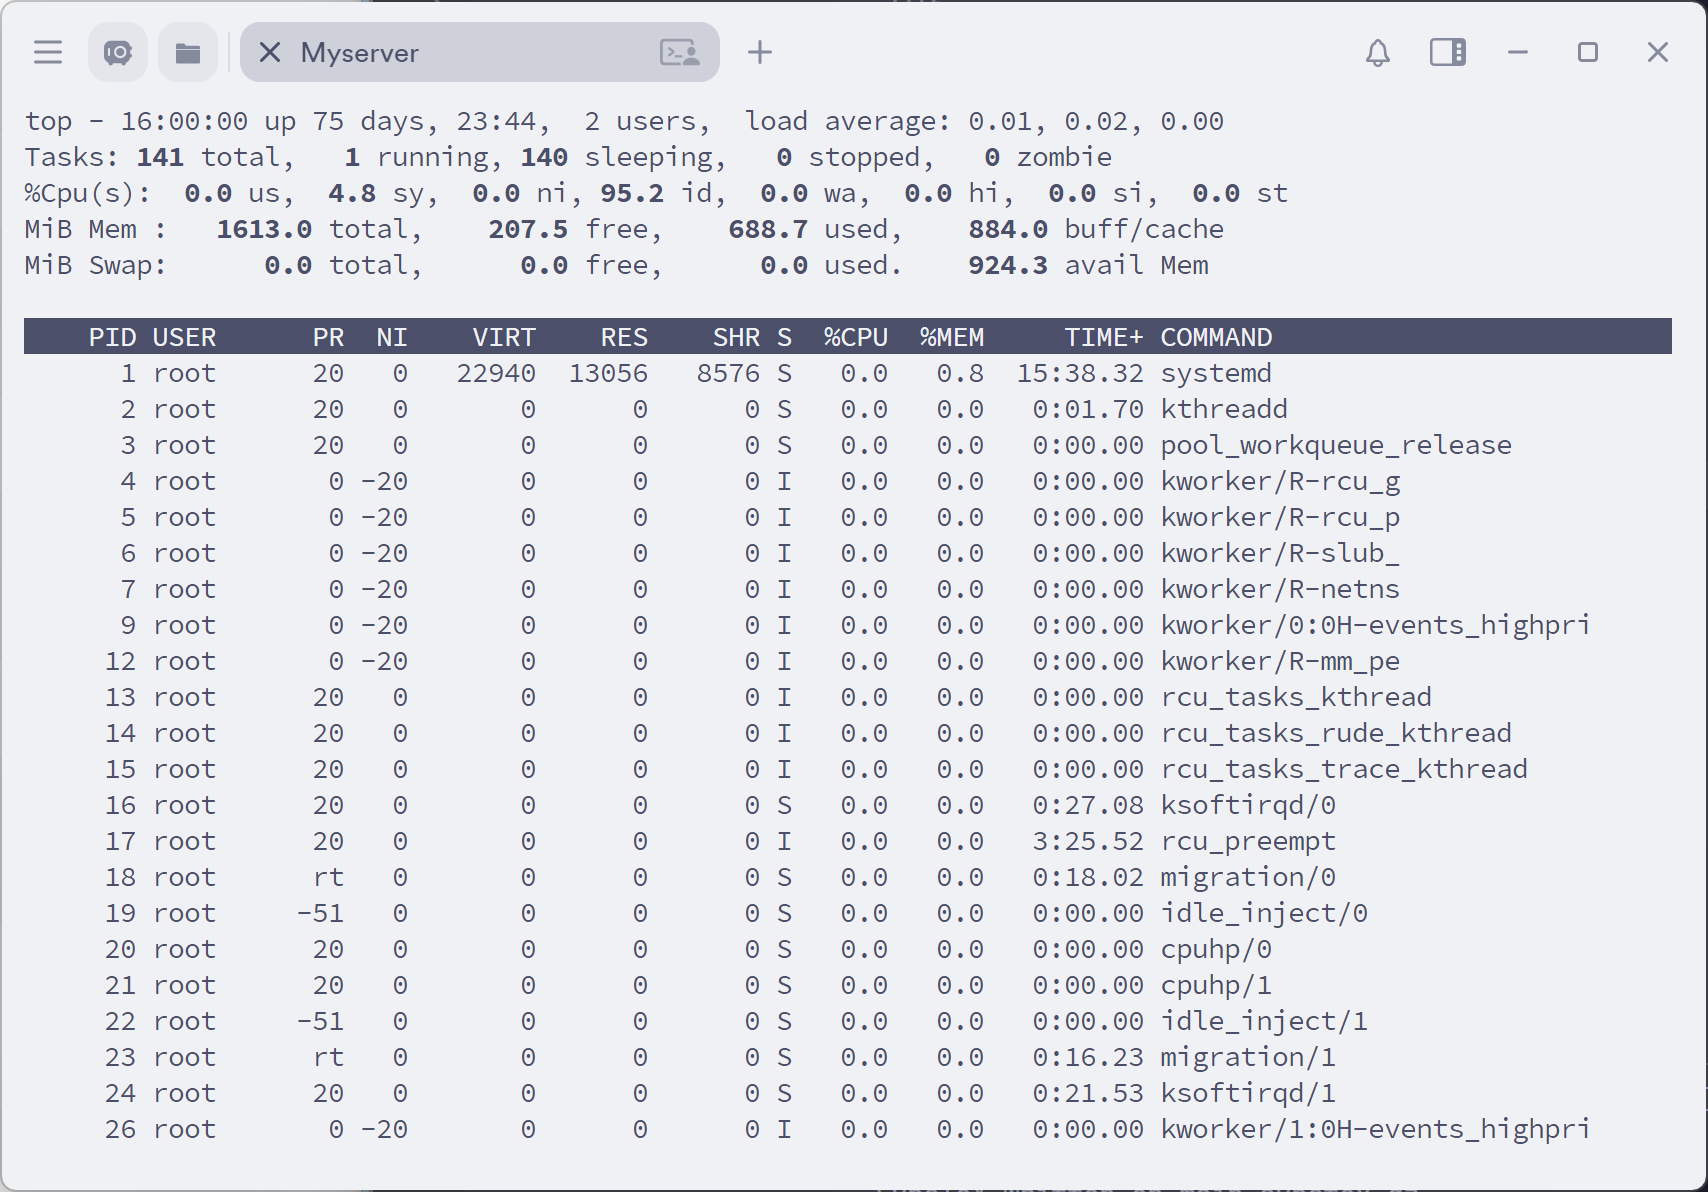
\includegraphics[width=0.8\textwidth]{pic/task1/image copy 8.png}
    \caption{命令3.7}
\end{figure}

\item 查看当前系统进程：\cmd{ps aux}

\begin{figure}[H]
    \centering
    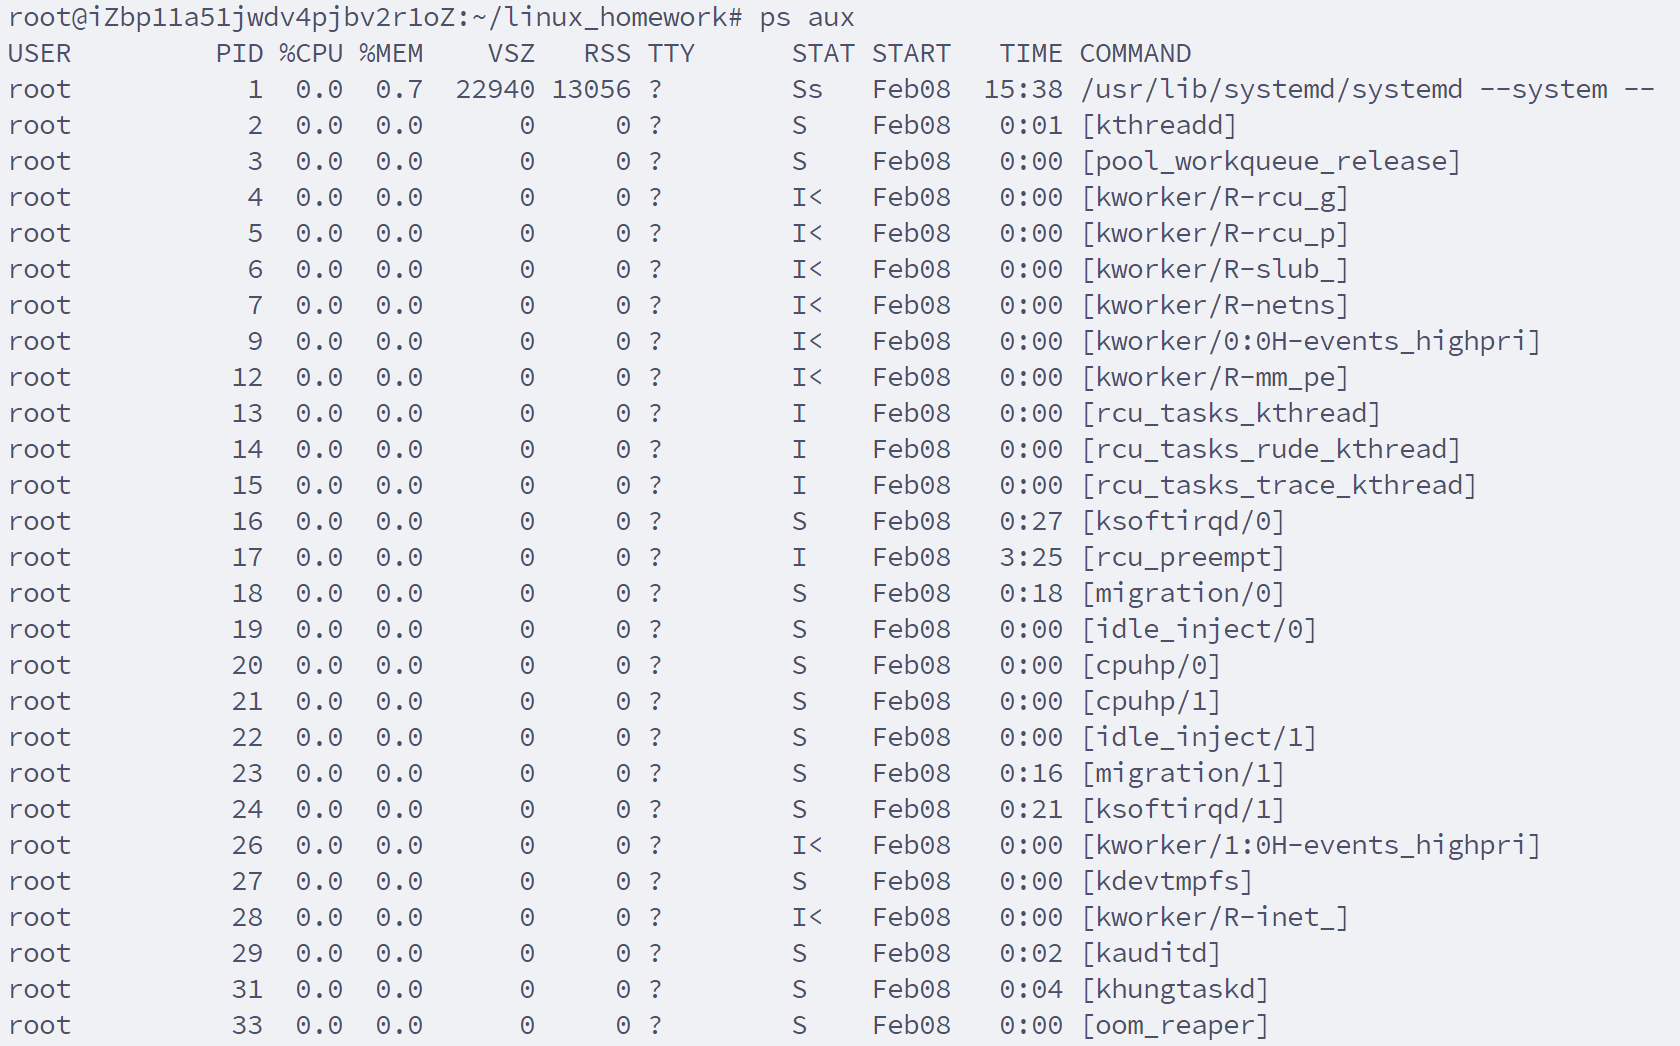
\includegraphics[width=0.8\textwidth]{pic/task1/image copy 9.png}
    \caption{命令3.8}
\end{figure}

由于使用的是远程服务器，系统进程比较多，截图中只保留了与本次演示相关的部分。

\item 查看历史命令：\cmd{history}

\begin{figure}[H]
    \centering
    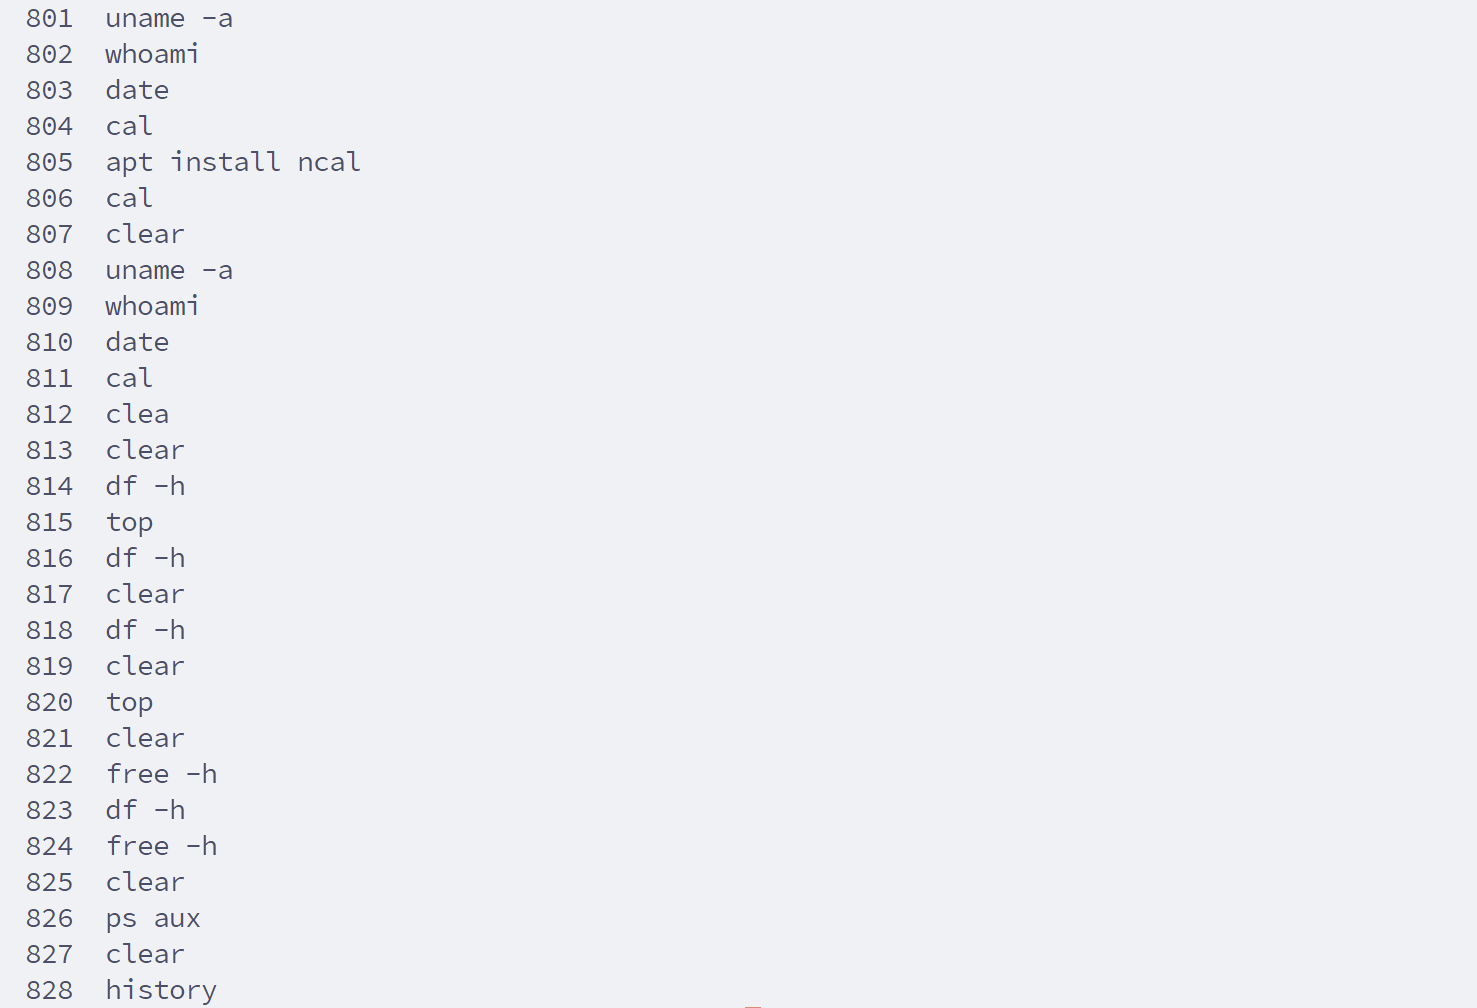
\includegraphics[width=0.8\textwidth]{pic/task1/image copy 10.png}
    \caption{命令3.9}
\end{figure}

历史记录中包含了我之前使用过的命令，包括一些测试命令和安装命令等。这里只截了本次课程展示的几个历史命令。

\end{enumerate}

系统信息命令的作用是帮助使用者判断“当前机器是什么状态”。例如 \cmd{df -h} 可以查看磁盘是否快满，\cmd{free -h} 可以查看内存余量，\cmd{ps aux} 和 \cmd{top} 可以观察进程数量和资源占用。对于服务器实验而言，这些命令尤其重要，因为远程环境没有图形化资源监视器，很多问题都需要通过命令行定位。

\begin{table}[H]
    \centering
    \caption{系统信息命令观察重点}
    \small
    \begin{tabular}{p{0.18\textwidth} p{0.30\textwidth} p{0.34\textwidth}}
        \toprule
        命令 & 主要观察对象 & 使用意义 \\
        \midrule
        \cmd{uname -a} & 内核版本、系统架构和主机信息 & 确认实验环境是否为目标 Linux 系统 \\
        \cmd{whoami} & 当前登录用户 & 判断是否拥有执行某些操作的权限 \\
        \cmd{date} & 当前系统时间 & 配合日志分析命令执行时间 \\
        \cmd{df -h} & 磁盘挂载点和空间使用 & 判断文件写入或编译失败是否与磁盘空间有关 \\
        \cmd{free -h} & 内存和交换空间使用 & 观察服务器是否存在内存压力 \\
        \cmd{ps aux} & 当前进程列表 & 查找正在运行的 shell、Python 或其他服务进程 \\
        \cmd{history} & 历史命令记录 & 复盘实验步骤，便于报告整理 \\
        \bottomrule
    \end{tabular}
\end{table}

\subsection{权限相关命令}

\begin{enumerate}
\item 创建脚本文件：\cmd{touch test.sh}
\item 查看文件权限：\cmd{ls -l test.sh}
\item 给文件添加可执行权限：\cmd{chmod +x test.sh}
\item 再次查看权限变化：\cmd{ls -l test.sh}
\item 查看文件详细状态信息：\cmd{stat test.sh}

\begin{figure}[H]
    \centering
    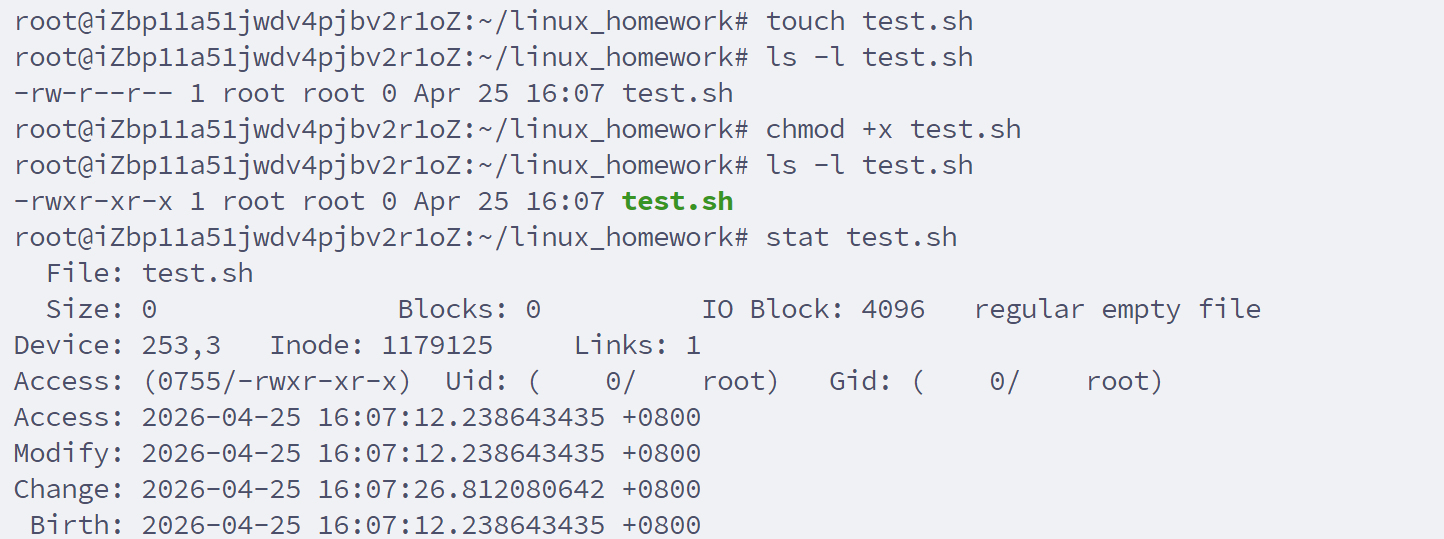
\includegraphics[width=0.8\textwidth]{pic/task1/image copy 11.png}
    \caption{命令4.1-4.5}
\end{figure}

\end{enumerate}

Linux 文件权限通常由三组权限组成，分别对应文件所有者、所属组和其他用户。每一组都可以包含读、写、执行三种权限，显示在 \cmd{ls -l} 输出的前十个字符中。例如普通文件的权限字段可能是 \cmd{-rw-r--r--}，第一个字符表示文件类型，后面九个字符按三组三位展示权限。脚本文件只有添加执行权限后，才可以直接通过 \cmd{./test.sh} 这样的形式运行。

\begin{table}[H]
    \centering
    \caption{权限字符与数字表示}
    \small
    \begin{tabular}{c c c p{0.38\textwidth}}
        \toprule
        权限 & 数字值 & 含义 & 常见影响 \\
        \midrule
        \cmd{r} & 4 & read，读取 & 可以查看文件内容或列出目录内容 \\
        \cmd{w} & 2 & write，写入 & 可以修改文件内容或在目录中创建、删除文件 \\
        \cmd{x} & 1 & execute，执行 & 文件可作为程序运行，目录可被进入 \\
        \cmd{-} & 0 & 无对应权限 & 操作会因权限不足失败 \\
        \bottomrule
    \end{tabular}
\end{table}

数字权限是把同一组中的读、写、执行权限相加得到的。例如 \cmd{7=4+2+1} 表示可读、可写、可执行，\cmd{5=4+1} 表示可读、可执行但不可写，\cmd{4} 表示只读。因此常见的 \cmd{chmod 755 script.sh} 表示所有者拥有全部权限，所属组和其他用户拥有读取与执行权限；\cmd{chmod +x test.sh} 则是在现有权限基础上给文件增加执行权限，更适合本次实验这种只需要让脚本可运行的场景。

\subsection{重定向与错误输出}

除了管道符，重定向也是 Linux 命令行中非常常见的数据流控制方式。管道符把前一个命令的标准输出交给后一个命令，而重定向则把命令的输入或输出连接到文件。本次实验中使用的 \cmd{echo "hello linux" > file1.txt} 就是一个输出重定向例子，它把原本应该显示在终端上的字符串写入文件。

\begin{table}[H]
    \centering
    \caption{常见重定向符号}
    \small
    \begin{tabular}{p{0.18\textwidth} p{0.28\textwidth} p{0.36\textwidth}}
        \toprule
        符号 & 含义 & 示例说明 \\
        \midrule
        \cmd{>} & 覆盖写入标准输出 & \cmd{echo hello > a.txt} 会覆盖原文件内容 \\
        \cmd{>>} & 追加写入标准输出 & \cmd{echo hello >> a.txt} 会把内容追加到文件末尾 \\
        \cmd{<} & 从文件读取标准输入 & 某些命令可以从指定文件中读取输入 \\
        \cmd{2>} & 重定向标准错误 & 把错误信息写入文件，便于排查失败原因 \\
        \cmd{2>\&1} & 将标准错误合并到标准输出 & 常用于同时保存正常输出和错误输出 \\
        \bottomrule
    \end{tabular}
\end{table}

理解标准输出和标准错误的区别，可以帮助定位脚本和命令执行失败的原因。普通结果一般通过标准输出显示，错误提示则通过标准错误显示。很多时候命令看起来“没有输出”，并不代表一定成功；也可能是输出被重定向到了文件，或者错误信息被单独写入了另一个位置。因此在写 Shell 脚本或运行批处理命令时，合理使用重定向可以保留运行记录，也能让后续调试更方便。

\subsection{管道符组合命令}

管道符 | 的作用是将前一个命令的输出结果作为后一个命令的输入。通过管道符，可以把多个简单命令组合成一个更复杂的数据处理流程。例如 \cmd{cat words.txt | sort | uniq -c | sort -nr} 先读取文件内容，再进行排序，然后统计重复行出现次数，最后按照出现次数从高到低排序，体现了 Linux 命令组合使用的灵活性。

\begin{enumerate}
\item 把文件内容传给 sort 排序后去重：\cmd{cat words.txt | sort | uniq}

\begin{figure}[H]
    \centering
    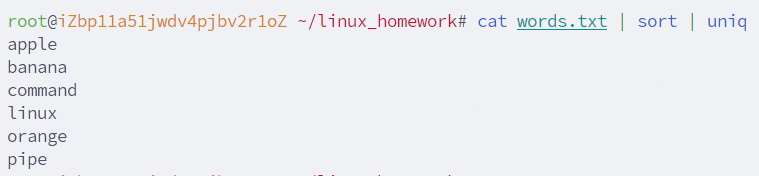
\includegraphics[width=0.8\textwidth]{pic/task1/image copy 12.png}
    \caption{命令5.1}
\end{figure}

\item 统计每个单词出现次数：\cmd{cat words.txt | sort | uniq -c}

\begin{figure}[H]
    \centering
    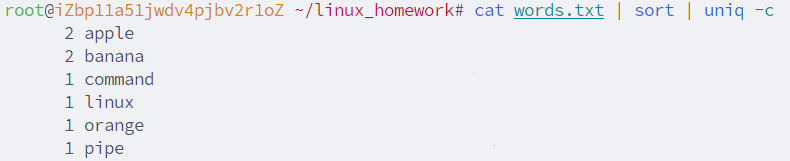
\includegraphics[width=0.8\textwidth]{pic/task1/image copy 13.png}
    \caption{命令5.2}
\end{figure}

\item 找出包含字母 a 的行，并排序：\cmd{grep "a" words.txt | sort}

\begin{figure}[H]
    \centering
    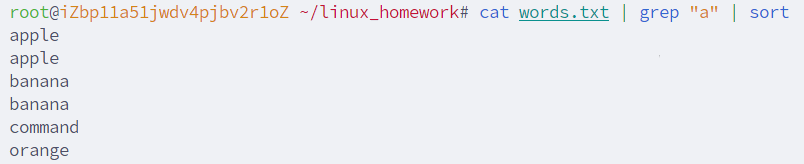
\includegraphics[width=0.8\textwidth]{pic/task1/image copy 14.png}
    \caption{命令5.3}
\end{figure}

\item 在当前目录中筛选 .txt 文件：\cmd{ls | grep '\textbackslash{}.txt\$'}
\item 在进程列表中查找 bash 相关进程：\cmd{ps aux | grep bash}
\item 查看最近使用的命令：\cmd{history | tail}

\begin{figure}[H]
    \centering
    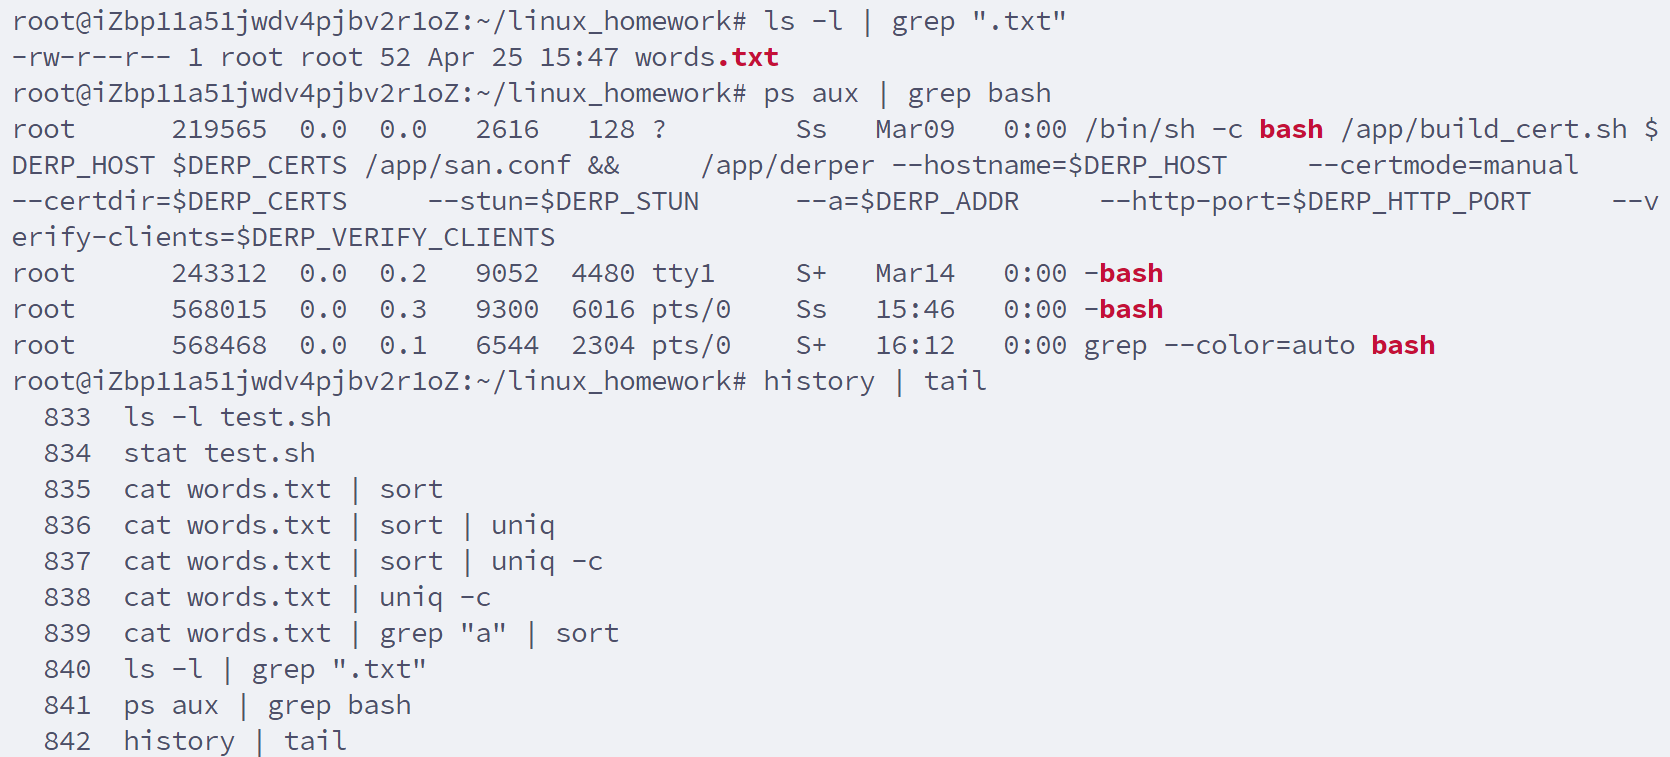
\includegraphics[width=0.8\textwidth]{pic/task1/image copy 15.png}
    \caption{命令5.4-5.6}
\end{figure}

\item 筛选磁盘挂载信息：\cmd{df -h | grep "/dev"}

\begin{figure}[H]
    \centering
    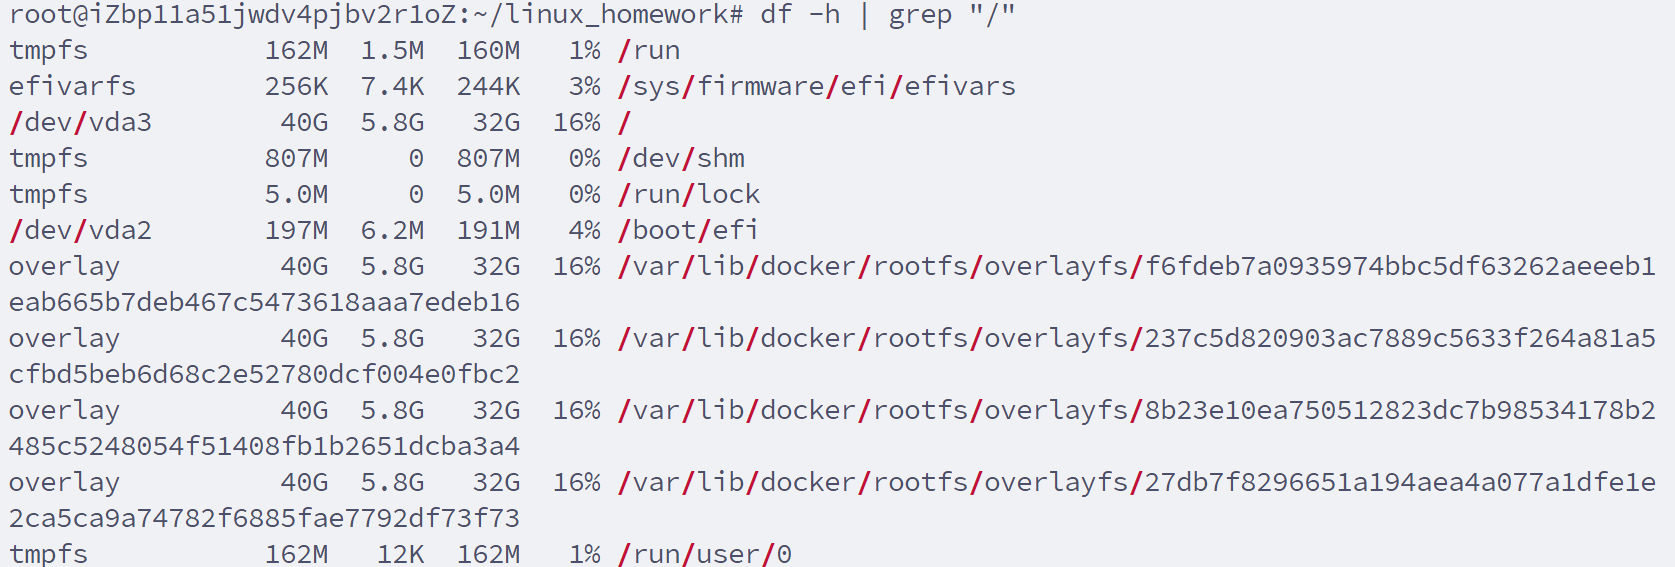
\includegraphics[width=0.8\textwidth]{pic/task1/image copy 16.png}
    \caption{命令5.7}
\end{figure}

\item 统计文件行数：\cmd{cat words.txt | wc -l}
\item 统计单词出现次数，并按出现次数从高到低排序：\cmd{cat words.txt | sort | uniq -c | sort -nr}

\begin{figure}[H]
    \centering
    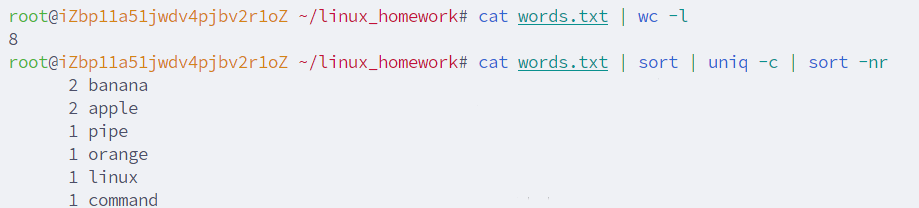
\includegraphics[width=0.8\textwidth]{pic/task1/image copy 17.png}
    \caption{命令5.8-5.9}
\end{figure}

\end{enumerate}

管道命令体现了 Linux 工具设计中的组合思想。每个命令只完成相对单一的任务，例如 \cmd{cat} 负责输出文件，\cmd{sort} 负责排序，\cmd{uniq -c} 负责统计相邻重复项，\cmd{sort -nr} 负责按照数字倒序排列。当这些命令通过管道连接后，就可以完成一个完整的词频统计流程。这种方式比把所有逻辑写进一个大型程序更灵活，也更容易在终端中快速试验。

\begin{table}[H]
    \centering
    \caption{管道组合命令的数据流}
    \small
    \begin{tabular}{p{0.24\textwidth} p{0.30\textwidth} p{0.30\textwidth}}
        \toprule
        命令片段 & 输入 & 输出 \\
        \midrule
        \cmd{cat words.txt} & 文本文件 & 原始单词列表 \\
        \cmd{sort} & 原始单词列表 & 按字典序排列后的行 \\
        \cmd{uniq -c} & 相邻重复内容 & 每个单词及出现次数 \\
        \cmd{sort -nr} & 带计数的行 & 按出现次数从高到低排列的结果 \\
        \cmd{grep "a"} & 多行文本 & 只包含字母 \cmd{a} 的行 \\
        \cmd{wc -l} & 多行文本 & 行数统计结果 \\
        \bottomrule
    \end{tabular}
\end{table}

\subsection{常见命令错误与排查}

在命令行实验中，错误信息本身也是学习内容。Linux 命令通常会明确告诉用户失败原因，例如文件不存在、权限不足、命令未安装或参数错误。遇到错误时，不应该只重新输入命令，而要先判断错误属于路径问题、权限问题、软件包问题还是命令格式问题。

\begin{table}[H]
    \centering
    \caption{常见错误与排查方法}
    \small
    \begin{tabular}{p{0.24\textwidth} p{0.28\textwidth} p{0.32\textwidth}}
        \toprule
        错误现象 & 可能原因 & 排查方法 \\
        \midrule
        \cmd{No such file or directory} & 路径写错或当前目录不对 & 使用 \cmd{pwd} 确认位置，用 \cmd{ls} 查看文件是否存在 \\
        \cmd{Permission denied} & 没有读写或执行权限 & 使用 \cmd{ls -l} 查看权限，必要时使用 \cmd{chmod} 修改 \\
        \cmd{command not found} & 命令未安装或名称拼写错误 & 检查命令拼写，必要时通过包管理器安装 \\
        删除后找不到文件 & \cmd{rm} 已经删除目标 & 删除前先用 \cmd{ls} 确认，重要文件先用 \cmd{cp} 备份 \\
        \cmd{uniq} 去重不完整 & 重复行没有相邻排列 & 先执行 \cmd{sort}，再执行 \cmd{uniq} \\
        管道结果为空 & 前一个命令没有输出或过滤条件太严格 & 分段执行管道，逐步检查每个命令的输出 \\
        \bottomrule
    \end{tabular}
\end{table}

这些排查方法也可以迁移到后面的 Shell 脚本和 Python 项目中。例如脚本无法执行时先看权限，文件读取失败时先看路径，网络服务无法访问时先确认进程是否运行和端口是否开放。命令行学习的价值不只是记住命令本身，更重要的是形成定位问题的顺序。

\subsection{综合命令练习复盘}

把前面几类命令组合起来，可以形成一个完整的小型文本处理任务。例如本次实验中的 \cmd{words.txt} 文件既可以用于查看内容，也可以用于排序、去重、统计和筛选。单独看每条命令时，它们只是简单操作；连起来看时，就能体现 Linux 命令行处理文本数据的能力。

\begin{minted}{bash}
cat words.txt | sort | uniq -c | sort -nr
\end{minted}

这条命令可以拆成四个阶段。第一阶段 \cmd{cat words.txt} 读取文件内容；第二阶段 \cmd{sort} 把相同单词排到相邻位置；第三阶段 \cmd{uniq -c} 统计每个相邻重复项的数量；第四阶段 \cmd{sort -nr} 按数字倒序排列统计结果。每个阶段都只完成一件事，但组合起来就得到了词频统计结果。

\begin{table}[H]
    \centering
    \caption{综合命令执行阶段分析}
    \small
    \begin{tabular}{p{0.18\textwidth} p{0.30\textwidth} p{0.34\textwidth}}
        \toprule
        阶段 & 命令 & 作用 \\
        \midrule
        读取数据 & \cmd{cat words.txt} & 把文本文件内容作为后续命令的数据来源 \\
        排序整理 & \cmd{sort} & 让相同内容相邻，为 \cmd{uniq} 做准备 \\
        统计次数 & \cmd{uniq -c} & 统计每个单词出现次数 \\
        结果排序 & \cmd{sort -nr} & 按出现次数从高到低排列，便于观察高频项 \\
        \bottomrule
    \end{tabular}
\end{table}

这种分阶段思维对后续 Shell 编程也很有帮助。写脚本时不一定要一次写出完整程序，可以先在命令行中把关键命令跑通，再把它们放进变量、循环和函数中。比如第二次作业中的历史成绩统计，本质上也是先读取成绩文件，再使用文本处理命令提取分数字段并计算最高分。

在实际使用中，我也发现管道命令的调试方式与普通程序类似：如果最终结果不对，就把管道从左到右拆开，一段一段执行。先确认原始输入是否正确，再确认排序结果，再确认统计结果，最后再看排序参数是否符合预期。这种调试方法简单但很有效，也体现了 Linux 命令组合的透明性。

\subsection{实验小结}

通过本次基础命令实验，我对 Linux 命令行的工作方式有了更系统的理解。文件和目录命令主要解决“在哪里”和“有什么”的问题，内容查看与处理命令用于观察和整理文本，系统信息命令帮助了解当前运行环境，权限命令则体现了 Linux 中文件可读、可写、可执行权限的基本模型。

其中管道命令给我的印象最深。单个命令的功能通常比较简单，但通过 \cmd{|} 可以把多个命令连接成完整的数据处理流程。例如排序、去重、计数和再次排序可以组合成一条命令完成词频统计。这体现了 Linux 工具“每个程序只做好一件事，再通过组合完成复杂任务”的思想，也为后续 Shell 脚本编程打下了基础。
